%!TEX root = ../Studienarbeit.tex

\section{Stand der Technik in der Tiervertreibung}

Um unliebsame Besucher aus dem Garten, Haus oder Auto zu vertreiben gibt es viele Geräte auf dem Markt. Zu diesen gehört ein großes Sortiment von Ultraschall-Tierschreck-Systemen, Sprinkleranlagen und verschieden Varianten von Weidezäunen. Um einen bestmöglichen Erfolg der Vertreibung zu bieten, sollen die Geräte an den Umschlagsorten der Tiere platziert werden.

Die einzelnen Systeme und deren Vor- und Nachteile werden in den nachfolgenden Unterkapiteln beschrieben.

\subsection{Ultraschall-Tierschreck} \label{ton_schreck}

Eine gängige Variante des Ultraschall-Tierschrecks ist der Marderschreck. Der Marderschreck wird in dem Motorraum eines Fahrzeugs platziert und soll verhindern, dass der Marder Schläuche und Kabel durchbeißt. Er verspricht das Fernhalten und Vertreiben der Tiere durch aussenden eines Hochfrequenztons. Der Ton hat dabei eine Frequenz von 17 bis 45 kHz. Für die Tiere ist dieser Frequenzbereich besonders unangenehm. Erwachsene Menschen nehmen diese Töne aber kaum bis gar nicht wahr. \cite{marderschreck}

Daher werden auch für den heimischen Garten diese Geräte gerne eingesetzt. Da sie aber nicht länger über die Autobatterie und der Lichtmaschine mit Energie versorgt werden, sind sie häufig an eine kleine Batterie und einem Solarpanel angeschlossen. Die gängigen Varianten eines Ultraschall-Tierschrecks für die Gartenverwendung haben zudem ein eingebautes Blitzlicht. Bei Nacht wird das Tier durch kurze Lichtimpulse zusätzlich beim Durchqueren des Gartens gestört und der Erfolg zur Vertreibung von nachtaktiven Tieren erhöht sich.
\\
Die Tiere, insbesondere Waschbären, gewöhnen sich allerdings an das Licht und dem Hochfrequenzton. Daher hält der Erfolg der Vergrämung oft nur wenige Wochen an.
Ultraschallgeräte können aber auch Probleme bereiten. Die eigenen Haustiere und auch Kleinkinder nehmen den Hochfrequenzton ebenso wahr. Da die Geräte auf jegliche Bewegung reagieren, kann es sein das der Ultraschall-Tierschreck vor Betreten des Gartens deaktiviert werden muss, damit die Haustiere und Kinder sich im Garten aufhalten können.\cite{anti_wasch}


\subsection{Automatische Sprinkleranlage} \label{sprinkler}

Eine andere Variante von Abschrecksystem ist der Einsatz von Sprinkleranlagen. Durch das Beschießen mit Wasser werden die Tiere besonders gut gestört. Der automatische Sprinkler wird über einen Bewegungsmelder ausgelöst und versprüht großflächig Wasser im Zielbereich. Nach eigener Erfahrung hat eine automatische Sprinkleranlage eine höhere Erfolgsquote, um ungewollte Besucher aus dem heimischen Garten zu vertreiben, aber sie kann durch den Bewegungsmelder auch unbeabsichtigt von einem selbst ausgelöst werden.\cite{anti_wasch}

Der Nachteil bei diesem System ist, dass der Sprinkler direkt mit einem Gartenschlauch verbunden werden muss. Dadurch treten deutliche Einschränkungen in der Positionierung des Abschrecksystems auf, da ein Wasseranschluss mit ausreichend Druck und Volumenstrom an ihm befestigt sein muss. Zusätzlich fällt der Druck und der Volumenstrom mit zunehmender Länge des Gartenschlauches ab, wie in den Artikel \textit{1/2 Zoll vs. 3/4 Zoll Gartenschlauch – Wann benötigt man welchen und welche Unterschiede gibt es?} aufgefallen ist. Der Author hat in diesem Artikel zwei verschieden Gartenschläuche und deren Druck- und Volumenstromverlust gemessen. Bei dem Test des Gartenschlauches mit 1/2 Zoll Durchmesser war nach zwei Metern bereits eine Reduzierung des Volumenstroms auf 62\% zu beobachten.\\

\comment{Selber noch überprüfen und bestätigen}
Angenommen ein eingesetzter Sprinkler hätte eine Düse mit einer Öffnung von 1,5 Millimeter in einer Höhe von einem Meter befestigt, so hätte die Reduzierung den Zielbereich von knappen 10 Metern auf 6 Meter reduziert.
Ein Sprinkler hätte somit mit zunehmender Entfernung proportional zum Volumenstrom an Reichweite verloren.

Ein anderer Punkt, der bei diesen Anlagen häufig vernachlässigt wird, ist die Verschwendung von Trinkwasser. Vor allem in Zeiten des Energie- und Wassersparens versucht man Verschwendungen zu minimieren. Einige Landkreise sind in den letzten Jahren in den Dürreperioden sogar so weit gegangen, dass das Rasensprengen aus eigener Quelle von 12 bis 18 Uhr verboten worden ist. Durch diese Maßnahmen erhofft man sich besser durch Dürreperioden zu kommen. Ein automatischer Rasensprinkler, der Trinkwasser verwendet sollte daher vermieden werden, um Dürreperioden nicht noch schlimmer zu machen.\cite{wasser_verbot}

\subsection{Weidezaun}

Der Weidezaun ist häufig das letzte Mittel um die Tiere aus dem Garten zu bekommen. Der Zaun wird um den Garten herum aufgebaut und sämtliche Durchgänge, an denen die Tiere in den Garten eindringen  können, sollen ebenfalls mit dem Zaun blockiert werden. Wenn das Getier nun versucht durch diese Zugänge in den Garten einzudringen, wird der Eindringling von dem Zaun einen schwachen elektrischen Schlag abbekommen.
\\
Ein Waschbär wird durch diesen Schlag in absehbarer Zeit es nicht noch einmal versuchen denselben Zugang zu verwenden. Häufig suchen die Tiere stattdessen einen anderen Zugang in den Garten. Wenn die Tiere keinen anderen Zugang zum Garten finden, wenden sie sich vom Grundstück ab. In unregelmäßigen Abständen überprüfen die Tiere allerdings ob die Blockade immer noch besteht. Der Weidezaun muss daher ständig eingeschaltet und gewartet werden.\cite{anti_wasch}

Der Weidezaun hat von den genannten Systemen die höchste Effektivität, wenn es um die Vertreibung der Tiere geht. Durch die Blockierung sämtlicher Zugänge besteht allerdings ein sehr hoher Installationsaufwand. Zusätzlich müssen weitere Elemente, wie Gartentore installiert werden, da sonst auch die Zugänge für den Menschen blockiert sind. Das gesamte System wird somit schnell teuer, weshalb der Weidezaun auch als letztes Mittel betrachtet wird.


\section{Computer Vision}

Computer Vision beschäftigt sich damit Computern das \enquote{Sehen} zu ermöglichen. Schon jahrzehntelang versuchen dies Wissenschaftler zu erreichen. Heutzutage sind sie schon sehr weit gekommen. Computer Vision findet in der Logistik, dem autonomen Fahren, Gesichtserkennung und bei noch vielen anderen Bereichen große Zuwendung. Ziel davon ist es Analysen, Verarbeitung und Interpretationen von Bildern und Videos durch einen Computer möglich zu machen, damit eine Maschinen visuelle Informationen so verstehen kann wie wir Menschen es tun. \cite{cv_Szeliski}

\subsection{Object Detection}

Object Detection ist eine Anwendung der Computer Vision, die es ermöglicht, Objekte in einem Bild oder Video zu erkennen und zu lokalisieren. Object Detection-Systeme verwenden Algorithmen, die auf \ac{ML}- und \ac{DNN}-Techniken basieren, um Objekte in Bildern oder Videos zu erkennen und zu klassifizieren. Das erkannte Objekt wird mittels einer \ac{BB} aus den Bild extrahiert. Beispiele für Objekterkennungen sind in Abbildung \ref{fif:ob_sample} abgebildet.
\\
Um diese Detektion zu erhalten gibt es verschieden Basen und Architekturen von Object Detections Systemen, die im folgenden beschreiben sind. \cite{cv_Szeliski}


\begin{figure}[h]
    \centering
    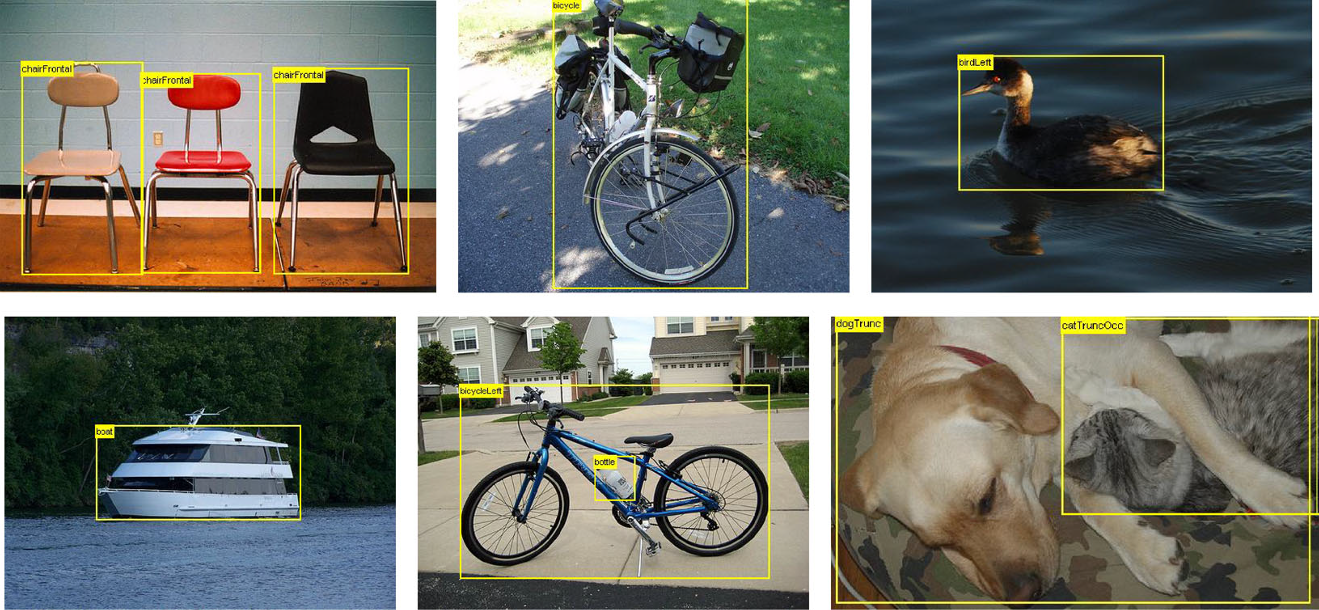
\includegraphics[width=\textwidth]{images/object_detection_sample.png}
    \label{fif:ob_sample}
    \caption{Beispiele für Objekt Erkennung und \acl{BB}. Quelle: \cite{cv_Szeliski}}
\end{figure}

\subsection{Two-Stage-Detectors}

Eins der frühen Modelle die diese Technik verwendet hat ist das \ac{R-CNN}. Es werden hirfür zwei große Schritte angewendet. Weshalb das \ac{R-CNN} und ähnliche Modelle als \textit{two-stage-Detectors} bezeichnet werden.\\
Der erste Schritt bei diesen Modellen ist es mittels eines \ac{RPN} rechteckige Regionen in einen Bild zu bestimmen.
Das \ac{RPN} schlägt hierbei eine Unterteilung des Eingabebildes in verschiedene Regionen vor. Das \ac{R-CNN}-Netzwerk lässt sich dabei ~2000 Regionen vorschlagen.
Aus diesen Regionen werden anschließend im zweiten Schritt die Feautures eines Eingabebildes durch ein \ac{CNN} extrahieren. Im Falle von \ac{R-CNN} werden die Feautures mittels einer Softmax-Schicht und einer \ac{SVM} ausgewertet und Objekte detektiert.\\
Dabei sollte die Anzahl der Regionen vernünftig klein sein, damit das nachfolgende extrahieren und klassifizieren in einer absehbarer Zeit erfolgt. Dieser zusätzliche Zeitaufwand, der für das \ac{RPN} aufgewandt wird, ist zudem auch ein Nachteil gegenüber anderen Ansätzen. Die Two-Stage-Detektoren erhalten dadurch zwar eine höhere Genauigkeit in der Lokalisierung und Klassifizierung, benötigen aber auch mehr Zeit.\cite{R_CNN}

\subsection{One-Stage-Detectors}

One-Stage Detektoren sind einer der neueren Ansätze Object-Detection zu realisieren.
Sie basieren auf die menschliche Natur und gehen von einer Single-Shot Erkennung aus. Dafür wenden sie entgegen den Two-Stage-Detektoren keinen Region-basierten Algorithmus an.
Stattdessen unterteilen sie ein Eingabebild in ein $S \times  S$ großes Gitternetz. Auf den Gitter-Boxen wird daraufhin ein Klassifizierung und Lokalisierung vorgenommen.\\
Dies war auch der erste Ansatz in der \ac{YOLO}-Architektur. Durch diesen Ansatz ist das \ac{YOLO}-V1 Modell entgegen den Two-Stage-Detektor Faster \ac{R-CNN} laut den Autoren in \cite{YOLO_V3} neun mal schneller bei der Detektierung. \ac{YOLO}-V1 ist aber deutlich schlechter, da deutlich weniger Objekte richtig detektiert worden sind. In Version 2 wird daher statt einem Gitternetz die Anchor-Boxen verwendet. Anchor-Boxen haben keine einheitliche Größe. Sie sind rechteckige Boxen, welche in verschiedenen Größen und Seitenverhältnissen angewendet werden. Die Anchor-Boxen werden auf einer Reihe von vordefinierten Positionen über ein Eingabebild verteilt.\\
Bei diesem Ansatz wird die Detektierung durch die Anchor-Boxen ermöglicht, ohne einen Verlust der Geschwindigkeit zu verursachen. Die Version 2 von \ac{YOLO} enthält noch andere Anpassungen, die die Anzahl an richtigen Detektionen weiter erhöht hat.
\cite{YOLO_V3}

Es gibt noch weitere nicht Anchor oder Gitter betriebene Architekturen, wie die \textit{CenterNet} oder \textit{CornerNet}-Architektur. Diese ermitteln den Mittelpunkt eines Objektes oder deren Kanten. Sie erhöhen die Präzession eines Detektors, benötigen aber wiederum mehr Ausführungszeit.\cite{yolo_all}

\subsection{Tiefenberechnung}

Für das Zielsystem ist es nötig den Abstand vom Objekt zur Zielvorrichtung zu ermitteln. Heutzutage gibt es \ac{ML}-basierte Techniken, die die Abstandsermittlung mit jeglicher Kamera durchzuführen können, aber es gibt einfachere und ältere Methode die Abstand zu einem Objekt zu bestimmen.
\\
Die meisten Lebewesen und wir Menschen haben eine einfache Möglichkeit dreidimensionale Strukturen zu erfassen und wahrzunehmen. Dabei setzen wir Menschen auf unsere zwei Augen. \textit{Stereo Vision} umfasst sich mit dem Bereich das binokulares Sehen von uns Menschen, um auch Computern es zu ermöglichen dreidimensional zu sehen.
\\
Dabei werden zwei Kameras verwendet, die gleichzeitig ein \textit{linkes} und ein \textit{rechtes} Bild aufnehmen. Die Kameras stehen dabei um eine kleine Abstand auch genannt \textit{Baseline} voneinander entfernt.
\\
Der Prozess zur Bestimmung der Tiefe erfolgt dann durch die Verwendung der epipolaren Geometry und Triangulation. Dabei betrachtet man einen Punkt im \textit{linken} Bild und den entsprechenden Punkt im \textit{rechten} Bild. Da die Kameras auf einer Höhe zueinander stehen, muss der Punkt nur auf der x-Achse, entlang der epipolaren Linie der beiden Kameras gesucht werden. Das ermitteln der passenden Punkte wird dabei als \textit{stereo matching} bezeichnet.
Aus der \textit{Baseline} und den Differenzpunkten zwischen den Koordinaten der einzelnen Bildern kann anschließend die Tiefeninformationen gewonnen werden. Das beschreiben Konzept ist in Abbildung \ref{fig:stereo_depth} zu sehen.
\\
Bei der Methode wird das Triangulieren zwischen den Punkten verwendet.
\cite{stereo_vision}

\begin{figure}[h]
    \centering
    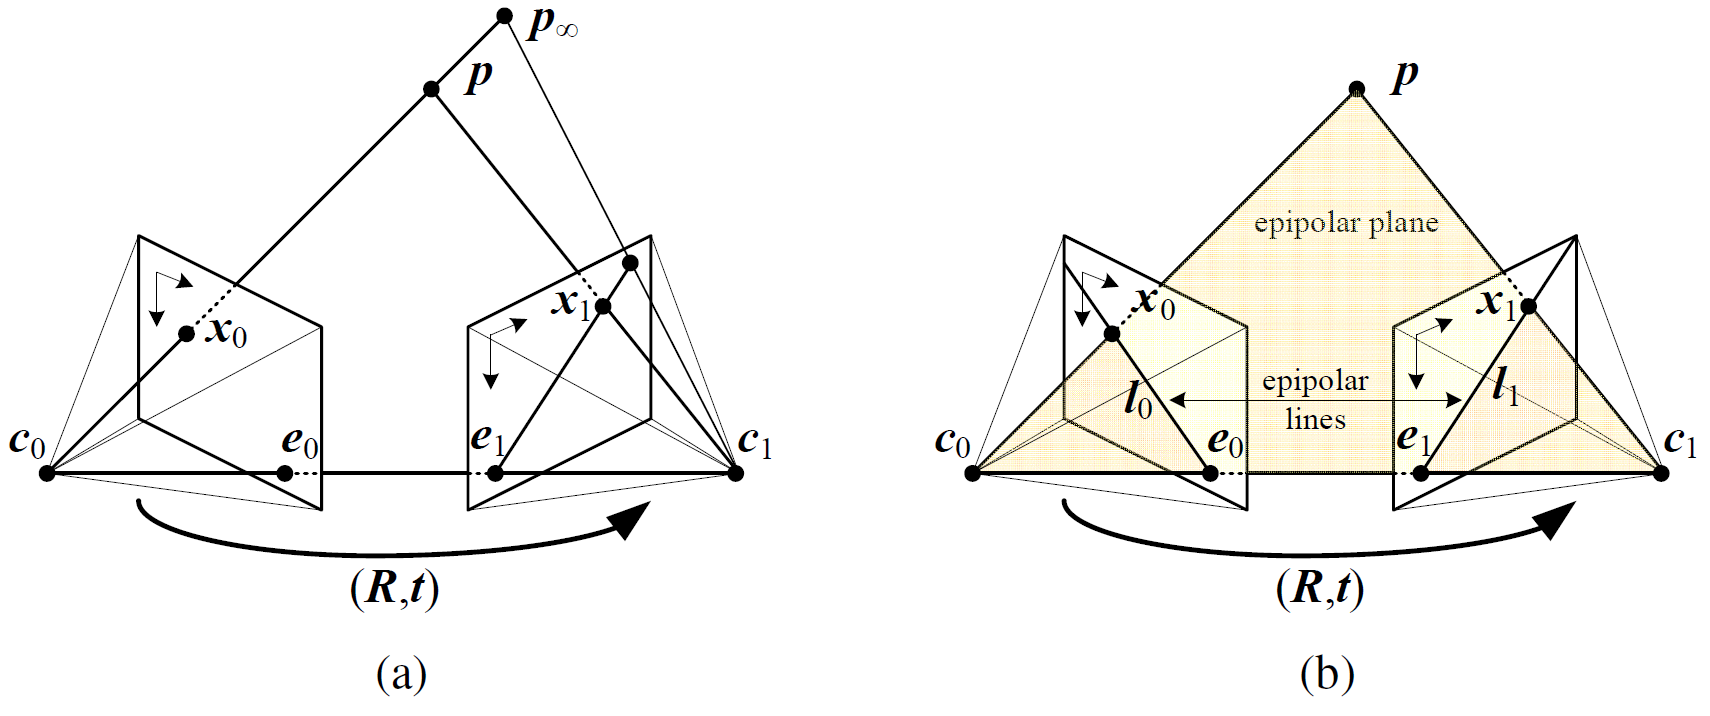
\includegraphics[width=\textwidth]{images/depth_sample.png}
    \label{fig:stereo_depth}
    \caption{(a) Epipolare Linie, die einen Lichtstrahl entspricht und (b die entsprechende epipolare Linien auf der Epipolarebene. Quelle: \cite{cv_Szeliski})}
\end{figure}

% Zusätzlich zu betrachtende Effekte Luftwiderstand; Dispersion; Wind/Error-correction etc.
% Bezug Error: Bilderkennung des Wasserstrahls $\rightarrow$ Regelungstechnik und Autokalibrierung
% + evtl. Einspielen der Tiefenwahrnehmung an neuer Position (nicht bei Stereo-Vision nötig).

\section{Komponenten}

Für die Realisierung eines portablen Abschrecksystems werden Aktoren und Komponenten benötigt, welche in diesem Kapitel beschrieben werden.

\subsection{Aktoren}

Das Abschrecksystem umfasst verschiedene Aktoren, die zur Vertreibung unliebsamer Kleintiere eingesetzt werden. Im Folgenden sind die Funktionen und Anforderungen der Aktoren sowie gegebenenfalls benötigte Zusatzelemente aufgelistet.

\subsubsection{Tonwiedergabe}

Waschbären, Marder und andere Tiere empfinden Hochfrequenztöne als äußerst unangenehm. Laut Westfalia \cite{westfalia_wasch} können Frequenzen im Bereich von 20 bis 40 kHz und ein Schalldruck von mindestens 100 dB bereits erfolgreich dazu beitragen, Waschbären zu vertreiben.

Gemäß den Informationen aus \cite{sound_amplifier} entspricht ein Watt leistungsaufnahme bei einem Meter Abstand vom Lautsprecher in etwa einem Schalldruck von 90 dB. Da die meisten Mikrocontroller nicht genug Leistung liefern können, um einen Lautsprecher mit höheren Leistungsanforderungen anzusteuern, wird ein Verstärker benötigt. Zusätzlich ist es erforderlich, dass das Abschrecksystem einen möglichst großen Radius abdecken kann, wodurch ein höheres Leistungsvermögen als die angegeben 100 dB erforderlich wird.

\subsubsection{Lichtimpulse}

Zusätzlich ist es sinnvoll Blinklichter zur visuellen Abschreckung einzusetzen. Da die meisten unliebsamen Tiere nachtaktiv sind, kann durch den stroboskopischen Effekt eine Vertreibung des Tieres erreicht werden. \cite{anti_wasch}

Auch hier können Mikrocontroller nicht das nötige Leistungsvermögen erbringen. Daher wird eine externe Energieversorgung und Schaltlogik benötigt.

\subsubsection{Wasserversorgung}

Wie in Kapitel \ref{sprinkler} beschrieben, haben sich Sprinkleranlagen als wirksam bei der Vertreibung von Tieren erwiesen. Da das System jedoch tragbar sein soll, ist es nicht möglich, einen Wasserschlauch anzuschließen. Zusätzlich muss der Wasserdruck ausreichend sein, um die Tiere in einem Radius von 10 Metern zu erfassen.
\\
Daher ist es erforderlich, eine Pumpe in das System einzubauen, die sowohl ausreichenden Druck als auch ausreichendes Pumpvermögen bietet. Die Pumpe muss ebenfalls von einer externen Stromversorgung und Schaltlogik gesteuert werden, da ein gezielter und leistungsstarker Einsatz erforderlich ist.

\subsubsection{Zielaktorik}

Für die Zielaktorik ist ein Zwei-Aktoren Zielsystem notwendig, welches horizontales und vertikales ansteuern von Zielwinkel ermöglicht. Elektromotoren eignen sich sehr gut für diese feinfühlige Ansteuerung. Allerdings gibt es große Unterschiede zwischen den verschieden Motortypen. Einige davon sind in folgender Tablelle \ref{tab:el_motors} beschrieben.

Hinzu kommt das die Motoren in ein dreidimensionales Zielsystem eingebaut werden. Daher sollte die Form und Größe ebenfalls betrachtet werden, da der Platz gering ist.

\begin{longtable}{ p{0.15\textwidth}|p{0.35\textwidth}|p{0.35\textwidth} }
    \endfirsthead
    \multicolumn{2}{l}%
    {\textit{Fortsetzung von vorheriger Seite}} \\
    \hline
    \endhead
    \hline \multicolumn{2}{r}{\textit{Fortsetzung auf nachfolgender Seite}} \\
    \endfoot
    \endlastfoot
    \textbf{Motortyp} & \textbf{Vorteile} & \textbf{Nachteile}\\
    \hline
    Schrittmotor &
    \begin{itemize}
        \item Einfache und präzise Ansteuerung möglich. Sie werden daher auch bei CNC-Fräsen und 3D-Drucker verwendet.
        \item Besitzen ein hohes Haltemoment.
        \item Berechnung der Position auch in der Open-Loop Steuerung möglich, da sie eine exakte Strecke pro Ansteuerungsschritt ermöglichen.
    \end{itemize}
    &
    \begin{itemize}
        \item Da sie einen inkrementelle Positionierung über die Schrittweite haben, müssen sie eventuell mit einem Getriebe untersetzt werden. Zum Beispiel würde bei einer Schrittweite von 1,8° beim Radius von 10 Metern pro Schritt 35 Zentimeter zurückgelegt werden. 
	\item Des weiteren kann es beim Zielvorgängen zu kurzzeitigen hohen Drehzahlen kommen. Der Schrittmotor verliert bei hohen Drehzahlen an Drehmoment und kann einzelne Schritte auslassen oder sogar stoppen.
    \end{itemize}
\\
    DC-Motor &
    \begin{itemize}
        \item Einfache Ansteuerung über \ac{PWM}.
        \item Hohes Drehmoment bei niedriger Drehzahl.
    \end{itemize}
    &
    \begin{itemize}
        \item H-Brücke nötig, da die Energie nicht über einen herkömmlichen Mikrocontroller geliefert werden kann.
        \item Motorsteuerung und Regelung notwendig.
        \item Sensoren werden benötigt, da eine Open-Loop Ansteuerung nur sehr geringe Genauigkeit bietet.
    \end{itemize}
    \\
    Servomotor &
    \begin{itemize}
        \item Keine Direkte Regelung nötig, da sie eine integrierte Closed-Loop Regelung haben.
        \item Sie können dynamisch auf hohe Belastung reagieren.
        \item Durch die Closed-Loop Regelung haben sie eine hohe Genauigkeit und keine zusätzlichen Bauelemente oder Treiberbauteile sind nötig.
    \end{itemize}
    &
    \begin{itemize}
        \item Häufig haben die erhältlichen Servomotoren nur einen geringen Positionsradius von 180°.
        \item Da sie konstant versuchen eine Sollposition zu erreichen kann es zu Jitter im System kommen.
    \end{itemize}
    \\
    \caption{Vergleich dreier Elektromotortypen für die Verwendung im Zielsystem. Quelle: \cite{motors_seed}}
    \label{tab:el_motors}
\end{longtable}


\subsection{Sensorik}

Der Aufgabenstellung entsprechend benötigt das System lediglich zwei optischen Sensoren, die in der Lage sind Bilder auch in der Nacht aufzunehmen.

Je nach Wahl der Aktoren können weitere Sensoren, wie Winkel- oder Stromsensoren im System verbaut sein. Da ein leistungsfähiger Mikrocontroller für die Object Detection verwendet werden soll, ist ein Temperatursensor für die Überwachung und zum Schutz vor Überhitzung zu empfehlen.

\subsection{3D-Druck}

Eine Realisierung eines vollständigen Prototyps des Abschrecksystems benötigt viel Zeit und Teile, die auf dem Markt nicht immer erhältlich, nicht auf den Anwendungsgebiet zugeschnitten oder sehr teuer sind.\\
Daher werden für das Abschrecksystem Einzelteile mittels CAD-Modellen und dem 3D-Drucker der DHBW hergestellt. Das ermöglicht eine schnelle auf dem Anwendungsgebiet zugeschnittene Herstellung von Einzelteilen zu günstigen Kosten.

Zudem hat die Firma softwareinmotion einen eigenen 3D-Drucker, der in den Praxisphasen für die Studienarbeit verwendet werden kann. Der Weg zur DHBW für das Abholen der 3D-Drucke wäre in den Praxisphasen nur schwer möglich gewesen.

Die CAD-Modelle werden mit der Autodesk Software \textit{Fusion 360} erstellt.

% \subsection{Strömungslehre}

% Pumpe $\rightarrow$ Nötigung anständiger Berechnung des Zielsystem

% \begin{equation} \label{v_qa}
%     v = Q/A
% \end{equation}

% \begin{equation}\label{Rohreibung}
%     \Delta p = \frac{\lambda \times L \times \rho \times Q^2}{2 \times A^2}
% \end{equation}

% mit Bernoulligleichung:

% \begin{equation}
%     \frac{v_{1}^2 \times \rho}{2} + p_1 = \frac{v_{2}^2 \times \rho}{2} + p_2 + \frac{\lambda \times L \times \rho \times Q^2}{2 \times A^2}
% \end{equation}

% da zunächst bei Hausleitung Druck ca. 4 Bar für $p_1$
